\chapter{Introduction}

\epigraph{
  Race de Caïn, au ciel monte,\\
  Et sur la terre jette Dieu !
}{---\textcite[16]{baudelaire-1857}}


\parencite{goguen-1991}

Category theory is a branch of mathematics developed in the 1940s
which has come to occupy a central position in computer science.


``Category theory is a relatively young branch of pure mathematics,
stemming from an area---algebraic topology---that most computer
scientists would consider esoteric. Yet its influence is being felt in
many parts of computer science, including the design of functional and
imperative programming languages, implementation techniques for
functional languages, semantic models of programming languages, models
of concurrency, type theory, polymorphism, specification languages,
constructive logic, automata theory, and the development of
algorithms'' \parencite[xi]{pierce-1991}.


``Developed in the 1940s as a way to organize constructs in algebraic
topology, category theory works at a level of whole mathematical
objects rather than their elements. (...) Category theory can be
viewed as a formalization of operations on abstract data types in
computer languages'' \parencite[1154]{wolfram-2002}.

``Category theory has come to occupy a central position in
contemporary mathematicas and theoretical computer science. Roughly,
it s a general mathematical theory of structures and of systems of
structures. As CT is still evolving, its functions are correspondingly
developing, expandind and multiplying'' \parencite[1]{marquis-2013}.
``Category theory thus affords philosophers and logicians much to use
and reflect upon'' \parencite[1]{marquis-2013}. ``From the 1980s to
the present, category theory has found new applications. In
theoretical computer science, category theory is now firmly rooted,
and contributes, among other things, to the development of new logical
systems and to the semantics of programming''
\parencite[23]{marquis-2013}.

``One does not so much learn category theory as absorb it over a
period of time'' \parencite[26]{bird-demoor-1997}.

``The trinity of concepts category, functor, and natural
transformation is what category theory is built on''
\parencite{nlab-category-theory}.

\paragraph{Theoretical framework and proposal}

Category theory is a relatively recent branch of mathematics which
occupies a central position en contemporary mathematics and
theoretical computer science. The object of study of category theory
are known as categories. Basically, a category is an aggregate of
objects and mappings (morphisms or arrows) between objects. The most
known example is the category Set, the category of sets and functions.
The definition of category is important to present some notions (such
as functors and natural transformations) which make category theory a
common tool which organizes and unifies many aspects of mathematics.
(Marquis 2010)

Some functional programming languages (such as Haskell) have certain
important concepts for relating category theory to programming. In
this sense, polymorphism, algebraic data types, and the functor and
monad type classes, etc., are concepts which can be conceptualized or
are based on ideas from category theory. Even if its categorical
conceptualization is not necessary for its use, it's an ideal
complement for better understanding functional programming and its
theoretical foundations. (Haskell community)

Polymorphism refers to the fact that the type of a value may depend on
the context in which it is used. Algebraic data types have various
alternatives or constructors of values. Type classes allow to define
generic interfaces which exhibit characteristics common to a great
variety of types. Finally, a functor (in Haskell) is a class of types
which can be mapped and a monad (of Haskell) is a class of types which
introduces the concepts of context and the use of normal functions
which preserve the contexts of those contexts. (Real World Haskell).

\paragraph{Justification}

The study of category theory allows to deepen scientific knowledge and
discover some of its practical applications to subjects that the
author has identified as important and interesting for his Systems
Engineering.

This project allows to study a topic related with computer science and
to deepen the study of theoretical foundations of the undergraduate.

The study of category theory will allow to understand and apply
effectively and efficiently the theoretical foundations of functional
programming. Category theory is a solid framework for a lot of
concepts of functional programming.

Even though the study of theoretical foundations of functional
programming is not strictly necessary for a programmer, it is an ideal
complement for his appropriate education and adequate understanding of
the theoretical and practical concepts of programming.

Category theory is a common tool which organizes and unifies many
aspects of mathematicals, which makes it an important tool for
studying the theoretical foundations of functional programming.

Category theory arises naturally in many areas of computer science and
programming (language design, formal semantics, type systems, et
cetera) (Hutton 2010), which makes it an important tool for studying
the foundations of some programming areas.

Even though the categorical formulation of some concepts may be
difficult to understand, category theory is a conceptual framework
which allows to deal with such concepts at a higher level of
abstraction.

\section*{Summary of the project}

This is an undergraduate project submitted in partial fulfillment of
the requirements for the degree of Systems Engineering at EAFIT. Here
is a summary of the project proposal, submitted in November 14, 2010.

Having this into account (that it is possible to conceptualize many
concepts of functional programming via the study of category theory,
this project aims to develop a monographical study of category theory
which allows to describe and explain some of the applications to
functional programming. In particlar, ...

Our goal (objective) is to describe and explain some of the
applications of category theory to functional programming. More
specifically, to describe and explain the concepts of category theory
which allow us to conceptualize and better understand the following
concepts of functional programming: polymorphism, algebraic data
types, and the functor and monad type classes.

The product or result of this project is a monograph on category
theory and some of its applications to functional programming. This
monograph contains the results of the development of the project, that
is, the results of the writing stage.

\section*{Audience and prerequisites}

We assume a working knowledge of functional programming in Haskell and
Agda. See the references on page
\pageref{sec:introduction-references}.

%% If any further background material is needed, it can be found in
%% textbooks on

The main audience of this project is any computer scientist with an
interest in mathematics, the theoretical foundations of computer
science or functional programming.

%% This book is addressed primarily to the mathematically inclined
%% functional programmer, though the non-functional -- but still
%% mathematically inclined -- programmer is not excluded. Although we
%% have taken pains to make the book as self-contained as possible, and
%% have provided lots of exercises for self-study, the reader will need
%% some mathematical background to appreciate and master the more
%% abstract material.

%% This project is written for mathematically inclined functional programmers.

%% The reader of this project is a mathematically inclined

%% We assume a working knowledge of functional programming in Haskell and
%% Agda.

%% The bibliographical remarks at the end of each chapter describe where
%% appropriate background material can be found.

\section*{Overview of the project} %% OR outline

This project is divided into six chapters organized like the tree
diagram in Figure \ref{fig:overview}:
\begin{itemize}
\item
  In Chapter \ref{chap:categories} (\nameref{chap:categories}), we
  define categories and commutative diagrams, and the categories which
  will allow us to relate category theory to functional programming in
  Haskell and Agda.

\item
  In Chapter \ref{chap:constructions} (\nameref{chap:constructions}),
  we describe some basic constructions in categories (isomorphisms,
  initial and terminal objects, and products and coproducts), which we
  use for describing some concepts and examples in all subsequent
  chapters.

\item
  In Chapter \ref{chap:functors} (\nameref{chap:functors}), we study
  functors and endofunctors in order to conceptualize and better
  understand functors in Haskell and Agda.

\item
  In Chapter \ref{chap:naturals} (\nameref{chap:naturals}), we explore
  the connection between natural transformations and polymorphic
  functions in Haskell.

\item
  In Chapter \ref{chap:monads} (\nameref{chap:monads}), we give a
  detailed account of monads and Kleisli triples, and their
  correspondence to monads in Haskell and Agda.

\item
  In Chapter \ref{chap:algebras} (\nameref{chap:algebras}), we
  describe algebras and initial algebras over endofunctors, and their
  relation to algebraic data types in Haskell.

\item
  Finally, Chapter \ref{chap:conclusions} (\nameref{chap:conclusions})
  contains our conclusions and some ideas for future work.

\end{itemize}

Each chapter, except Chapter \ref{chap:constructions}, is further
subdivided into two or three sections concerning some concepts of
category theory, and their relation to functional programming in
Haskell and, in some cases, Agda. Additionally, each chapter ends with
a References section which collects the sources of information for all
definitions and examples.

\begin{figure}[htb]
  \begin{center}
    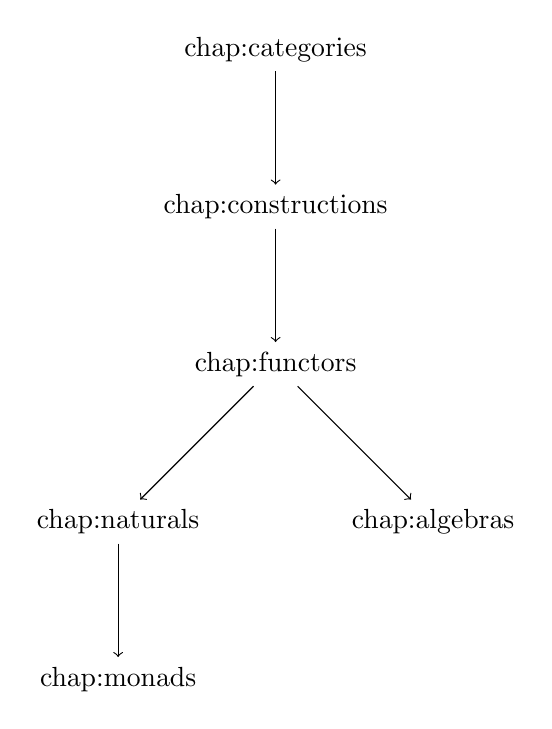
\begin{tikzpicture}
      \node (categories)    at (2,8) {\nameref{chap:categories}};
      \node (constructions) at (2,6) {\nameref{chap:constructions}};
      \node (functors)      at (2,4) {\nameref{chap:functors}};
      \node (naturals)      at (0,2) {\nameref{chap:naturals}};
      \node (monads)        at (0,0) {\nameref{chap:monads}};
      \node (algebras)      at (4,2) {\nameref{chap:algebras}};

      \draw [->] (categories)    to (constructions);
      \draw [->] (constructions) to (functors);

      \draw [->] (functors)      to (naturals);
      \draw [->] (naturals)      to (monads);

      \draw [->] (functors)      to (algebras);
    \end{tikzpicture}
  \end{center}
  \caption{Overview of the project.}
  \label{fig:overview}
\end{figure}

\section*{References}
\label{sec:introduction-references}

\paragraph{Category theory}

\begin{itemize}
\item
  Most of our definitions are based on \parencite{maclane-1998}, which
  is the standard reference on category theory.

\item
  \parencite{marquis-2013}, which includes: general definitions,
  examples, and applications; brief historical sketch; philosophical
  significance; and a programmatic reading guide. A useful
  programmatic reading guide can be found in
  \parencite[48--56]{marquis-2013}.

  It is an introductory and philosophical article regarding general
  category theory. Nice article for the preliminary study of category
  theory and contains an extended annotated bibliography.

\item
  The following book provides an accessible approach to category
  theory and categorical logic: \parencite{awodey-2010}

\item
  \parencites{eilenberg-maclane-1942}{eilenberg-maclane-1945}

\item
  \parencite{bird-demoor-1997} is a standard reference on the
  applications of category theory to computer science. Some parts of
  the book were used for the project proposal.

\item
  \parencite{pierce-1991} is an introductory reference for studying
  the applications of category theory to computer science. It is a
  summary of category theory and some of its applications, and
  contains a detailed bibliography.

  And \parencite[§ 4]{pierce-1991} contains books and articles for
  further reading.

\item
  \parencite{poigne-1992} is a reference for studying the applications
  of category theory to computer science. This book was the main
  reference for the project proposal.

\item
  Reprints in Theory and Applications of Categories
  \url{http://www.tac.mta.ca/tac/reprints/} including
  \parencites{adamek-et-al-2006}{barr-wells-2005}{barr-wells-2012}

\end{itemize}

\paragraph{Haskell}

\begin{itemize}
\item
  \parencites{lipovaca-2011}{osullivan-et-al-2008} or the
  HaskellWiki\footnote{\url{http://www.haskell.org/}}

  %%  Learn You a Haskell for Great Good! A Beginner's Guide

  %% RWH is an easy-to-use, fast-paced tutorial that introduces to
  %% Haskell.

\item
  \parencites{elkins-2009}{yorgey-2009}

  %% Typeclassopedia is a starting point for the student of Haskell
  %% wishing to gain a firm grasp of its standard type classes. The
  %% essentials of each type class are introduced, with examples,
  %% commentary, and extensive references for further reading.

  %% Elkins. Several concepts in Haskell are inspired by or taken from
  %% category theory. The most notable example being monads. tools for
  %% analyzing and building monads and related structures.

\end{itemize}

\paragraph{Agda} Sd

\begin{itemize}
\item
  The Agda wiki.\footnote{\url{http://wiki.portal.chalmers.se/agda/}}
  \parencite{norell-2007}

\item
  \parencites{bove-dybjer-2009}{norell-2009}

\end{itemize}

\paragraph{Sd}

\begin{itemize}
\item
  \parencite{weisstein-mathworld}

\item
  $n$Lab

\end{itemize}

\section*{Notes}

\paragraph{Frontispiece}

The illustration in page \pageref{fig:hatter}, John Tenniel's
\emph{Hatter engaging in rhetoric}, is taken from the Tenniel
illustrations for Lewis Carroll's \emph{Alice's Adventures in
  Wonderland}\footnote{\url{http://www.gutenberg.org/ebooks/114}.}.

\paragraph{Haskell and Agda code}

\begin{itemize}
\item
  Haskell code was tested with GHC 7.6.3.

\item
  Agda code was tested with Agda 2.3.2.2 and the Agda standard library
  0.7.

\end{itemize}

\paragraph{Links}

\begin{itemize}
\item
  This document is available for download at
  \url{http://bit.ly/1cq5fwN}.

\item
  A printable version is available at \url{http://bit.ly/1hDomqv}.

\item
  In addition, all Agda examples can be found in the repository
  \begin{center}
    \url{https://github.com/jpvillaisaza/abel}
  \end{center}

\end{itemize}
For more information, send an email to
\href{mailto:jvillai@eafit.edu.co}{\nolinkurl{jvillai@eafit.edu.co}}.

\clearemptydoublepage
